\documentclass[a4paper,14pt]{extarticle}

\usepackage[a4paper,top=20mm,bottom=20mm,left=30mm,right=10mm]{geometry}
\usepackage[T1,T2A]{fontenc}
\usepackage[utf8]{inputenc}
\usepackage[russian]{babel}
\usepackage{indentfirst}
\usepackage{titlesec}
\usepackage{graphicx}
\usepackage{verbatim}
\usepackage{fancyvrb}

\renewcommand{\baselinestretch}{1.3}
\titleformat{\section}{\normalsize\bfseries}{\thesection}{1em}{}
\titleformat{\subsection}{\normalsize\bfseries}{\thesection}{1em}{}
\setlength{\parindent}{12.5mm}

\begin{document}

  \newpage\thispagestyle{empty}
  \begin{center}
    \MakeUppercase{
      Министерство науки и высшего образования Российской Федерации\\
      Федеральное государственное бюджетное образовательное учреждение высшего образования\\
      <<Вятский Государственный Университет>>\\
    }
    Институт математики и информационных систем\\
    Факультет автоматики и вычислительной техники\\
    Кафедра электронных вычислительных машин
  \end{center}
  \vfill

  \begin{center}
    Отчет по лабораторной работе №2.2\\
    по дисциплине\\
    <<Управление данными>>\\
    <<Основы DML-запросов в PostgreSQL>>\\
  \end{center}
  \vfill

  \noindent
  \begin{tabular}{ll}
    Выполнил студент гр. ИВТб-2301-05-00 \hspace{5mm} &
    \rule[-1mm]{25mm}{0.10mm}\,/Макаров С.А./\\
    
    Преподаватель & \rule[-1mm]{25mm}{0.10mm}\,/Клюкин В.Л./\\
  \end{tabular}

  \vfill
  \begin{center}
    Киров 2025
  \end{center}

  \newpage
  \section*{Цель}
  Цель лабораторной работы: освоить основные варианты DML-запросов в PostgreSQL, научиться создавать SQL-скрипты для заполнения таблиц данными, познакомиться с типами данных в PostgreSQL, освоить основные варианты DDL-запросов в PostgreSQL, научиться использованию команды update и delete, научиться работать с представлениями.

  \section*{Задание}
  \begin{enumerate}
    \item Создать и выполнить SQL-скрипт, который будет заполнять таблицы данными. Нужно добавить не менее 3-5 строк в каждую таблицу.
    \item Создать представления для нескольких таблиц, в которых собираются данные из самой таблицы и других, на которые она ссылается. Выборка из любого представления должна давать полную и осмысленную информацию по сущностям. Хотя бы одно из представлений должно быть сделано с использованием соединений (join) в запросе
  \end{enumerate}

  \pagebreak
  \section*{Решение}
  Создадим представление, которое будет отображать минимальное значение, максимальное значение, среднее значение, сумму значений. Результат выборки представлен на рисунке 4. Соотвествующий SQL-скрипт представлен ниже:

  \noindent
  \begin{Verbatim}[tabsize=4,fontsize=\small]
CREATE OR REPLACE VIEW "ingredients_price_metric_v" AS

SELECT
    'Минимальное значение' as metric,
    MIN(price) as price,
    (SELECT id FROM "ingredients" ORDER BY price ASC LIMIT 1) as id
FROM "ingredients"

UNION ALL

SELECT
    'Максимальное значение',
    MAX(price),
    (SELECT id FROM "ingredients" ORDER BY price DESC LIMIT 1)
FROM "ingredients"

UNION ALL

SELECT
    'Среднее значение',
    ROUND(AVG(price)),
    NULL
FROM "ingredients"

UNION ALL

SELECT
    'Сумма значений',
    SUM(price),
    NULL
FROM "ingredients";

SELECT * FROM "ingredients_price_metric_v";
  \end{Verbatim}

  \begin{figure}[h]
    \centering
    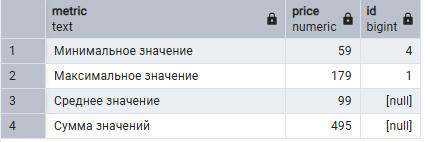
\includegraphics[width=0.75\linewidth]{img/view-1}
  \end{figure}
  \begin{center}
    Рисунок 4 – Результат выборки представления
  \end{center}

  \section*{Вывод}
  В ходе выполнения лабораторной работы изучены основы DML-запросов в PostgreSQL, такие как запросы на вставку данных, запросы на выборку и создание представлений. Исходя из вышеописанного созданы запросы на вставку данных, созданы представления с выборкой данных с соединениями с другими таблицами.

\end{document}